% This must be in the first 5 lines to tell arXiv to use pdfLaTeX, which is strongly recommended.
\pdfoutput=1
% In particular, the hyperref package requires pdfLaTeX in order to break URLs across lines.

\documentclass[11pt]{article}

% Change "review" to "final" to generate the final (sometimes called camera-ready) version.
% Change to "preprint" to generate a non-anonymous version with page numbers.
\usepackage[review]{acl}

\usepackage[most]{tcolorbox} % For creating colored and styled boxes

\usepackage[utf8]{inputenc}
\usepackage{multirow}
\usepackage{booktabs}

\usepackage{pgfplots}
\pgfplotsset{compat=1.17}
\usepackage{tikz}
\usetikzlibrary{arrows.meta,positioning,shapes.geometric,fit}

% Standard package includes
\usepackage{times}
\usepackage{latexsym}

% For proper rendering and hyphenation of words containing Latin characters (including in bib files)
\usepackage[T1]{fontenc}
% This is not strictly necessary, and may be commented out,
% but it will improve the layout of the manuscript,
% and will typically save some space.
\usepackage{microtype}

% This is also not strictly necessary, and may be commented out.
% However, it will improve the aesthetics of text in
% the typewriter font.
\usepackage{inconsolata}

% Including images in your LaTeX document requires adding
% additional package(s)
\usepackage{graphicx}

\usepackage{amsmath}
\usepackage{amssymb}
\usepackage{array}
\usepackage{url}

\title{STACHE: Stratified, Typed-Claim, Agreement-Gated, Cross-Condition Hallucination Evaluation for Clinical LLM Faithfulness on TCGA-LUAD}

\author{Anonymous ACL submission}

\begin{document}
\maketitle

\begin{abstract}
Clinical-LLM faithfulness evaluations typically report one number (the rate of bundle-supported claims), which cannot distinguish a model that reads the bundle from one whose priors match the cohort. We introduce \textbf{STACHE}, a \textbf{S}tratified-cohort, \textbf{T}yped-claim, \textbf{A}greement-gated, \textbf{C}ross-condition \textbf{H}allucination \textbf{E}valuation methodology instantiated on 119 TCGA-LUAD cases. STACHE pairs grounded and ungrounded generation, reports the Hallucination Dependence Index (HDI; fraction of ungrounded hallucination suppressed by grounding), and uses embedding overlap to separate calibrated uncertainty from prior-recycling. The harness pairs a rule-based checker with a fixed external LLM judge on sealed multimodal bundles, validated against a two-expert 300-claim consensus ($\kappa=0.64$). Across gpt-4o-mini, gpt-5.4-mini, gemini-2.5-flash, and gemini-3-flash-preview, HDI ranges 0.336--0.984 while grounded support compresses to 81.9--93.2\%, inverting rankings: grounded-only scoring prefers gemini-2.5-flash (93.2\%) over gemini-3-flash-preview (81.9\%), yet gemini-3 fabricates on 91.5\% of ungrounded cases versus 64.8\% for gemini-2.5. OpenAI's generational pair moves opposite (16.0\% $\to$ 5.9\%); gpt-5.4-mini's low HDI (0.336) reflects calibrated refusal, not prior-recycling (3.2\% overlap). STACHE+HDI thus identifies when grounding prevents clinical-LLM hallucination.
\end{abstract}

\section{Introduction}
\label{sec:intro}

Hallucination is a central concern for clinical applications of large language models. When a model writes ``pathology shows CD274 at 4.2 TPM, consistent with moderate immunotherapy response,'' a clinician cannot tell from the sentence whether the number came from the patient's record or from the model's prior over TCGA-LUAD. Strong LLMs encode clinical knowledge \citep{singhal2023largelanguagemodelsencode} yet produce unfaithful generations under evidence constraints \citep{ji2023survey,maynez2020faithfulness,pal2023medhalt}. The standard faithfulness evaluation, a single supported-claim rate against an evidence bundle \citep{deyoung2021ms2,tsatsaronis2015bioasq}, cannot distinguish a model that reads the bundle from one whose priors already match the cohort: both can score 87\% while differing in clinical safety. This ambiguity can only be diagnosed by running the same model without the bundle and observing the delta.

We use \textbf{grounded} to mean the configuration in which an LLM receives a sealed evidence packet for the patient, in the spirit of retrieval-augmented generation \citep{lewis2020rag,shuster2021retrieval}: pathology, RNA, clinical notes, and a fused immune tier \citep{thorsson2018immune}. We use \textbf{ungrounded baseline} to mean the same prompt with only a case ID (e.g.\ \texttt{TCGA-44-6147}) and cohort name (\texttt{TCGA-LUAD}). The ungrounded condition is a direct hallucination probe: any specific claim there is fabricated by construction. Medical-RAG work shows retrieval benefit is non-monotone across backbones \citep{xiong2024benchmarking}; we extend that from multiple-choice QA to open-ended oncology summarization.

We build a clinical oncology tooling stack \citep{collisson2014comprehensive} around this experimental design: a sealed multimodal evidence-bundle builder, a keyword-gated conditional PubMed retriever, a provider-agnostic chat layer, a claim extractor, and a dual checker pairing rule-based value-matching with a fixed external LLM-as-judge, chosen to avoid the self-preference artifact reported by \citet{panickssery2024llm}. STACHE is the full methodology instantiated on this apparatus: 119 TCGA-LUAD cases, a four-condition generation protocol, the dual checker (validated against a 300-claim human anchor, $\kappa = 0.64$), and a diagnostic panel of two metrics, the Hallucination Dependence Index (HDI) and semantic claim overlap. Across a 2\,$\times$\,2 factorial (gpt-4o-mini, gpt-5.4-mini, gemini-2.5-flash, gemini-3-flash-preview), STACHE surfaces three findings a grounded-only evaluation would miss: HDI ranges 0.336--0.984 while grounded support rate compresses to 81.9--93.2\%; the newer Google model produces unsupported claims on more of its ungrounded generations than its older sibling (91.5\% vs 64.8\%), contrary to the aligned-tuning intuition \citep{ouyang2022training}; and semantic overlap via \texttt{text-embedding-3-small} \citep{openai2024embeddings} indicates that gpt-5.4-mini's low HDI reflects calibrated priors rather than silent recycling.

Our contributions are:
\begin{itemize}
\item \textbf{STACHE}, a \textbf{S}tratified-cohort, \textbf{T}yped-claim, \textbf{A}greement-gated, \textbf{C}ross-condition \textbf{H}allucination \textbf{E}valuation methodology for clinical LLM faithfulness, with four coupled methodological choices (Section~\ref{sec:hqb}): (a) a paired grounded-vs-ungrounded protocol with the Hallucination Dependence Index (HDI) and a semantic claim-overlap probe; (b) stratified-within-tier cohort sampling that anchors each phenotypic stratum to a different reference point; (c) agreement-gated two-pass LLM judging with disagreement recorded as an explicit \texttt{conflict} label and excluded from the judge rate; and (d) type-conditioned rule-based verification over a six-class claim typology. STACHE is anchored to a 300-claim two-expert human adjudication.
\item A \textbf{provider-agnostic clinical evaluation stack} engineered as a controlled instrument that operationalizes STACHE end-to-end. Its novelty is in the set of design choices that make the paired contrast measurable and fair, not in any one component: (i) \emph{sealed} multimodal JSON evidence bundles (pathology, RNA, clinical, fused immune tier) that fix the LLM's information state (no free-text retrieval, no chain-of-thought scratchpad) so the grounded/ungrounded contrast is a true difference in evidence access rather than a difference in context shape; (ii) a matched grounded/ungrounded prompting protocol in which prompt template, system message, tool surface, and decoding parameters are held constant and only the bundle is substituted, making HDI a controlled measurement; (iii) a keyword-intent-gated PubMed retriever, repurposing retrieval as a \emph{measured discipline signal} (fired-when-requested vs.\ false-positive firing) instead of an unobserved confound; (iv) a provider-agnostic chat layer that enforces cross-provider parity (shared 120s timeout after observing silent socket hangs in the google-genai SDK, shared exponential-backoff retry on 429/5xx, fixed generation $T{=}0.2$ and judge $T{=}0$), making OpenAI-vs-Google comparisons fair by construction; (v) a dual checker combining type-aware rule-based matching (claims tagged \texttt{numeric}, \texttt{modality}, \texttt{tier}, \texttt{uncertainty}, \texttt{literature} with type-specific verification logic) with a fixed external LLM-as-judge (gpt-4.1-mini, in neither factorial row), which removes the \citet{panickssery2024llm} self-preference confound by construction rather than by correction; and (vi) a determinism envelope (fixed seeds, models, temperatures, embedding model, and cohort split) that makes the entire pipeline replayable end-to-end.
\item \textbf{Empirical findings STACHE makes visible} on 119 TCGA-LUAD cases, run as a 2\,$\times$\,2 factorial of four frontier LLMs: grounded support rate and HDI produce inverted rankings; HDI alone conflates two clinically distinct failure modes (overt confabulation vs calibrated-prior coverage) that the overlap probe separates; and the cross-condition factorial surfaces a within-provider divergence in ungrounded behavior invisible to grounded-only metrics.
\end{itemize}

\section{Related Work}
\label{sec:related}

\paragraph{Biomedical summarization and medical RAG.}
BioASQ \citep{tsatsaronis2015bioasq} and MS$^2$ \citep{deyoung2021ms2} established evidence-grounded biomedical QA and multi-study summarization, and Med-HALT \citep{pal2023medhalt} and Med-PaLM \citep{singhal2023largelanguagemodelsencode} have probed medical LLM hallucination at scale. Retrieval augmentation reduces hallucination in knowledge-intensive generation \citep{lewis2020rag,shuster2021retrieval}; MedRAG \citep{xiong2024benchmarking} extends this to medical QA across 41 corpus/retriever/LLM combinations and finds that retrieval benefit is non-monotone across backbones. The biomedical faithfulness literature has operated almost exclusively on a single-model, grounded-output regime; no prior clinical benchmark contrasts grounded and ungrounded conditions of the same model at factorial scale.

\paragraph{LLM-as-judge biases and hallucination taxonomy.}
Strong LLM judges \citep{zheng2023judging} correlate with human preference but exhibit position, verbosity, and self-enhancement bias; \citet{panickssery2024llm} show GPT-4 can recognize and favor its own generations at $\sim$73.5\% accuracy. These findings motivate our single fixed external judge. On the faithfulness side, \citet{ji2023survey} and \citet{maynez2020faithfulness} formalize the intrinsic/extrinsic split; our two failure modes (Section~\ref{sec:discussion}) layer an evaluation-centered dimension on top, distinguishing high-baseline confabulation from low-baseline calibrated-prior coverage.

\paragraph{Positioning of STACHE.}
STACHE's four pillars draw selectively from this prior work and make targeted departures. The paired \emph{cross-condition} protocol generalizes the standard RAG ablation \citep{lewis2020rag,shuster2021retrieval,xiong2024benchmarking} from a side comparison into a primary diagnostic axis with a single-number metric (HDI), measured under matched prompting rather than reported as a contrastive table. The fixed external judge addresses the self-preference bias of \citet{panickssery2024llm} in within-family MT-Bench-style protocols \citep{zheng2023judging}; STACHE further departs from majority-vote multi-pass judging by recording pass-to-pass disagreement as an explicit \texttt{conflict} label excluded from the headline judge rate, turning judge instability into a measured reliability signal rather than averaging it away. \emph{Stratified-within-tier} sampling with three tier-specific sort keys (descending for Hot, distance-to-center for Warm, ascending for Cold) anchors each phenotypic stratum to a distinct reference point; we are not aware of an equivalent intra-tier sort discipline in published clinical LLM evaluation, where uniform random or single-key stratified sampling is standard. \emph{Type-conditioned} rule-based verification over a six-class clinical claim typology, with per-type tolerances (numeric bands, modality-presence checks, adjacent-tier partial credit), departs from single-rule faithfulness checkers \citep{maynez2020faithfulness} that apply uniform string-match or entailment logic regardless of claim semantics. To our knowledge, STACHE is the first faithfulness methodology to present these four choices as a single coupled instrument.

\section{System}
\label{sec:system}

Our clinical oncology tooling stack is a modular pipeline for reproducible cross-model hallucination evaluation in the oncology setting. Figure~\ref{fig:system} summarizes the data flow; this section describes each component.

\begin{figure}[t]
\centering
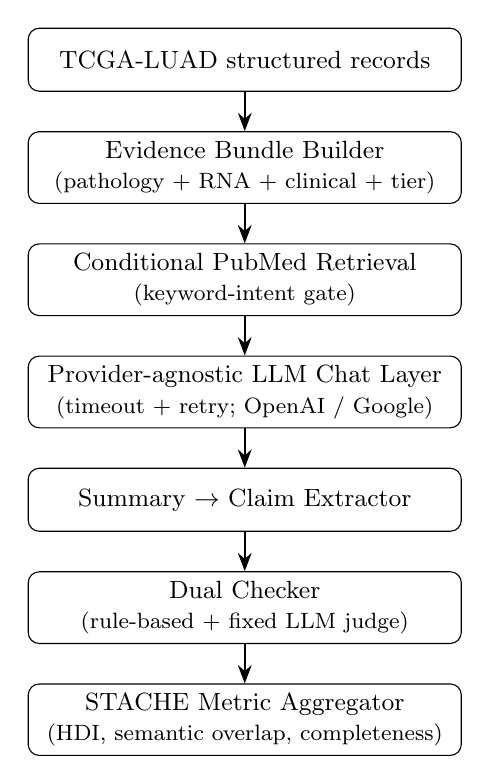
\begin{tikzpicture}[
  node distance=0.5cm and 0.5cm,
  box/.style={draw, rounded corners, minimum width=5.5cm, minimum height=0.8cm, align=center, font=\small},
  arrow/.style={->, >=Stealth, thick},
]
\node[box] (tcga) {TCGA-LUAD structured records};
\node[box, below=of tcga] (bundle) {Evidence Bundle Builder \\ \footnotesize (pathology $+$ RNA $+$ clinical $+$ tier)};
\node[box, below=of bundle] (retriever) {Conditional PubMed Retrieval \\ \footnotesize (keyword-intent gate)};
\node[box, below=of retriever] (llm) {Provider-agnostic LLM Chat Layer \\ \footnotesize (timeout $+$ retry; OpenAI / Google)};
\node[box, below=of llm] (summary) {Summary $\rightarrow$ Claim Extractor};
\node[box, below=of summary] (checker) {Dual Checker \\ \footnotesize (rule-based $+$ fixed LLM judge)};
\node[box, below=of checker] (panel) {STACHE Metric Aggregator \\ \footnotesize (HDI, semantic overlap, completeness)};

\draw[arrow] (tcga) -- (bundle);
\draw[arrow] (bundle) -- (retriever);
\draw[arrow] (retriever) -- (llm);
\draw[arrow] (llm) -- (summary);
\draw[arrow] (summary) -- (checker);
\draw[arrow] (checker) -- (panel);
\end{tikzpicture}
\caption{Clinical oncology tooling stack. Structured TCGA-LUAD records flow through a sealed bundle builder, an optional keyword-gated literature retriever, and a provider-agnostic LLM chat layer into a dual-checker faithfulness evaluator. STACHE is the top-level methodology and aggregator that produces the Hallucination Dependence Index (HDI) and semantic claim-overlap numbers.}
\label{fig:system}
\end{figure}

\paragraph{Evidence bundle builder.}
For each case the builder assembles a closed JSON bundle comprising four data layers: pathology (tumor/stroma/necrosis percentages, tile-level scoring, TIL density annotation when present), RNA (TPM values for a curated panel of immunotherapy-relevant genes including CD274, PDCD1, CTLA4, TIGIT, LAG3, HAVCR2, IDO1, CD8A, CD8B, GZMB, PRF1, IFNG, plus housekeeping normalizers), clinical (stage, age, sex, smoking history, prior therapy), and a pre-computed IO immune tier (Hot/Warm/Cold) derived from transcriptomic tertiles following the logic of \citet{thorsson2018immune}. The bundle is \emph{sealed} in the sense that the prompt to the LLM carries only this JSON; no open-ended free-text retrieval and no chain-of-thought scratchpad access.

\paragraph{Conditional PubMed retrieval.}
A lightweight keyword-intent classifier decides whether to invoke PubMed retrieval for a given generation request. Queries such as ``what does the literature say about PD-L1 IHC thresholds in LUAD'' fire retrieval; queries such as ``is this patient likely to respond to IO therapy'' do not. This gate lets us measure retrieval false-positive rate (literature fired when not requested) as part of our STACHE discipline metrics. In our evaluation the gate exhibits a 1.0 fired-when-requested rate and a 0.0 false-positive rate across all four models.

\paragraph{Provider-agnostic LLM chat layer.}
A single \texttt{chat()} wrapper dispatches to OpenAI's Chat Completions API or Google's \texttt{google-genai} SDK transparently. Three engineering choices ensure comparability across providers: (i) a per-request timeout of 120 seconds on both providers, introduced after we observed silent socket hangs in the google-genai Python SDK under sustained load; (ii) exponential-backoff retry on HTTP 429, HTTP 5xx, and network-class exceptions, shared across providers; and (iii) generation temperature fixed at 0.2 for all models and judge temperature fixed at 0.0 for consistency across two-pass scoring.

\paragraph{Claim extractor and dual checker.}
Each summary is split into sentence-level claims through a deterministic parser: a sentence tokenizer that respects medical-abbreviation boundaries (\texttt{Stage III.}, \texttt{IHC 3+.}, \texttt{N0/M0.}) feeds a lightweight regex pass that tags each claim as one of six types (\texttt{numeric}, \texttt{modality}, \texttt{tier}, \texttt{uncertainty}, \texttt{literature}, or \texttt{other}), with multi-tag inheritance when a sentence contains more than one signal (e.g., a numeric value attributed to RNA picks up both \texttt{numeric} and \texttt{modality}). Each tagged claim is then evaluated by two independent checkers. The rule-based checker matches numeric and enumerated values against the bundle with $\pm 0.01$ tolerance for rounded floats and $\pm 1$ percentage point for integer percentages, and produces one of \{supported, partial, unsupported, unknown\}. The LLM-as-judge (gpt-4.1-mini, $T{=}0$, two independent passes; the final label equals the pass-1 label when the two passes agree and is otherwise recorded as the explicit value \texttt{conflict} and excluded from the judge-supported rate) reads claim and bundle in natural language and votes supported / partial / unsupported. The two checkers are complementary: the rule-based checker is paraphrase-strict but deterministic (moderate human agreement, $\kappa{=}0.43$) and reproducible across runs; the judge is paraphrase-aware and substantially agreeing with humans ($\kappa{=}0.64$, Section~\ref{sec:validation}). Fixing the judge externally (gpt-4.1-mini is in neither the OpenAI nor the Google factorial row) removes the self-preference confound of \citet{panickssery2024llm} by construction; no generating model evaluates its own output.

\paragraph{STACHE metric aggregator.}
Consumes the judged \texttt{claim\_review.csv} to compute auto-supported rate, judge-supported rate, judge agreement, modality attribution accuracy, numeric fidelity, per-configuration completeness, retrieval discipline, HDI (Section~\ref{sec:methods}), and, via a separate OpenAI text-embedding-3-small pass \citep{openai2024embeddings}, semantic claim overlap. All metrics are deterministic given fixed model identifiers, fixed temperatures, fixed embedding model, and fixed seeds in the cohort selection script.

\section{Methodology}
\label{sec:methods}

\subsection{Cohort}
We evaluate on 119 TCGA-LUAD lung adenocarcinoma cases \citep{collisson2014comprehensive}. The full LUAD cohort is sorted by our multimodal immune-tier score and partitioned into tertiles (Hot / Warm / Cold); 119 cases are selected with approximately equal representation across tertiles so that evaluation does not reduce to a single phenotype. Cohort selection is deterministic: seeds and scripts fixed.

\subsection{Models}
The 2\,$\times$\,2 factorial covers two LLM providers and two model generations per provider. OpenAI: \texttt{gpt-4o-mini} (older) and \texttt{gpt-5.4-mini} (newer). Google: \texttt{gemini-2.5-flash} (older) and \texttt{gemini-3-flash-preview} (newer). All runs were executed in April 2026; generation temperature is 0.2, top-p default; prompt text is held bit-for-bit identical across providers via the provider-agnostic chat layer.

\subsection{Four-condition generation protocol}
Each case is generated under four configurations of our clinical oncology tools: (i) \texttt{pathology\_only}: bundle restricted to the pathology layer; (ii) \texttt{pathology\_rna}: pathology plus RNA; (iii) \texttt{full\_multimodal}: pathology, RNA, clinical, and tier all present; (iv) \texttt{ungrounded\_baseline}: the model receives only the case identifier and cohort name, with the same generation prompt. Configurations (i)--(iii) vary the \emph{depth} of grounding; configuration (iv) removes grounding entirely, and is the direct hallucination probe: any specific claim produced here is fabricated by construction.

\subsection{Judge validation against human adjudication}
\label{sec:validation}
To validate the GPT-4.1-mini judge, two of the authors, both domain experts, jointly labelled by consensus a stratified random sample of 300 claims (60 per model-condition bucket, covering 5 of the 8 factorial cells) drawn blind from \texttt{claim\_review.csv}, with the judge and rule-based labels withheld during annotation. Disagreements between the two annotators were resolved by discussion before a final label was recorded; the reported human label is therefore a two-expert consensus rather than a single-annotator judgment. We chose consensus labeling to maximize label quality on a small adjudication sample; the tradeoff is that an independent inter-human $\kappa$ cannot be recovered from this protocol, and we return to that limitation in Section~\ref{sec:limitations}. Table~\ref{tab:agreement} reports inter-rater agreement. The judge achieves $\kappa = 0.64$ against human labels (substantial agreement on the Landis-Koch scale), with a bootstrap 95\% CI of $[+0.55, +0.72]$. The rule-based checker reaches only moderate agreement with human labels ($\kappa = 0.43$), consistent with its known paraphrase-intolerance. We therefore treat the two checkers as complementary rather than ranked: HDI and the Results headlines are reported on the rule-based label because it is the more conservative, deterministic, and mechanically reproducible signal (single code path, no sampling variance, no vendor dependency), and the fixed LLM judge is retained as a paraphrase-aware cross-check against rule-based false negatives. Cross-model conclusions are drawn only where both checkers move in the same direction; neither is designated primary.

\begin{table}[h]
\centering
\small
\setlength{\tabcolsep}{4pt}
\resizebox{\columnwidth}{!}{%
\begin{tabular}{lccc}
\toprule
\textbf{Rater pair} & \textbf{Raw agr.} & \textbf{$\kappa$} & \textbf{95\% CI} \\
\midrule
Human vs.\ rule-based        & 0.63 & 0.43 & {[+0.39, +0.47]} \\
Human vs.\ GPT-4.1-mini      & 0.72 & 0.64 & {[+0.55, +0.72]} \\
Rule-based vs.\ GPT-4.1-mini & 0.54 & 0.42 & {[+0.23, +0.49]} \\
\bottomrule
\end{tabular}}
\caption{Inter-rater agreement on a stratified 300-claim human adjudication sample ($N=300$, 60 claims per model-condition bucket). $\kappa$ is Cohen's kappa; CIs are 1000-resample bootstrap. Landis-Koch: $\kappa \geq 0.61$ = substantial.}
\label{tab:agreement}
\end{table}

\subsection{The Hallucination Dependence Index (HDI)}
Let $u_b$ denote the unsupported-claim rate in the ungrounded baseline condition and $u_g$ the unsupported-claim rate in the grounded full-multimodal condition, each measured on the rule-based auto label. Define:
\begin{equation}
\text{HDI} = \frac{u_b - u_g}{u_b}, \quad u_b > 0.
\label{eq:hdi}
\end{equation}
HDI is the fraction of a model's ungrounded hallucination that the grounded architecture suppresses. HDI ranges over $[-\infty, 1]$ in principle, but meaningfully over $[0, 1]$ for any model whose grounded hallucination rate does not exceed its ungrounded rate. HDI is undefined when $u_b = 0$; we treat this as an edge case not observed in our data. HDI is distinct from supported-rate delta: a model with a very low baseline unsupported rate cannot show a high absolute delta, but can still show a high HDI if the relative reduction is large.

\subsection{Semantic claim overlap}
The HDI captures the \emph{amount} of hallucination suppressed but not whether the grounded model is generating genuinely case-specific content or merely paraphrasing baseline-style claims. We probe the latter directly with semantic claim overlap. For each patient, each grounded and baseline claim is embedded using OpenAI \texttt{text-embedding-3-small} \citep{openai2024embeddings}. For each grounded claim we compute its maximum cosine similarity to any baseline claim from the same patient; if the maximum exceeds $\tau$, the grounded claim has a \emph{semantic twin} in the baseline. The patient-level semantic overlap is the fraction of grounded claims with a semantic twin, averaged over the cohort. We report $\tau = 0.80$ (the standard paraphrase threshold) as the primary number and $\tau \in \{0.75, 0.85\}$ for sensitivity. Embedding-based semantic similarity cannot distinguish ``PD-L1 is low'' from ``PD-L1 is high'' (same clinical topic, opposite magnitudes) and therefore biases overlap \emph{upward}; low overlap values are therefore robust evidence of genuine content divergence.

\subsection{Scope of novelty}
\label{sec:hqb}
The four methodological choices in the preceding subsections and the system section (cross-condition HDI with semantic-overlap probe, stratified-within-tier cohort sampling, agreement-gated two-pass judging, and type-conditioned rule-based verification) compose into \textbf{STACHE} as a single coupled instrument rather than four independent improvements. No component is algorithmically novel in isolation; the contribution is their joint instantiation on a clinical cohort and the diagnostic payoff that combination produces. Section~\ref{sec:related} positions each pillar against prior work, and the contributions list (Section~\ref{sec:intro}) names the six engineering choices in the surrounding stack that make the panel reproducible across providers. The panel makes three findings visible that no grounded-only benchmark can produce: grounded support rate and HDI yield inverted rankings on the same four models; HDI alone conflates two clinically distinct failure modes (Mode A vs Mode B, Section~\ref{sec:discussion}) that the overlap probe separates; and the cross-condition factorial exposes within-provider divergence in ungrounded behavior. Any existing clinical-LLM faithfulness suite can adopt STACHE by adding one ungrounded-baseline run, the HDI computation, and the overlap probe; we release the harness, prompts, cohort split, and evaluator.

\section{Results}
\label{sec:results}

\begin{table*}[!t]
\centering
\small
\begin{tabular}{lrrrrr}
\toprule
\textbf{Model} & \textbf{Baseline sup.} & \textbf{Baseline unsup.} & \textbf{Grounded sup.} & \textbf{Grounded unsup.} & \textbf{Judge agree} \\
\midrule
gpt-4o-mini             & 79.6\% & 16.0\% & 84.4\% & 0.2\%  & 0.683 \\
gpt-5.4-mini            & 87.7\% & 5.9\%  & 87.7\% & 4.0\%  & 0.720 \\
gemini-2.5-flash        & 33.0\% & 64.8\% & 93.2\% & 5.2\%  & 0.970 \\
gemini-3-flash-preview  & 7.5\%  & 91.5\% & 81.9\% & 14.0\% & 0.794 \\
\bottomrule
\end{tabular}
\caption{2\,$\times$\,2 factorial. ``Baseline'' refers to the ungrounded condition (model receives only case ID and cohort), ``Grounded'' to the full\_multimodal condition. Supported and unsupported rates are on the rule-based auto checker; judge-agreement is the two-pass self-consistency of the fixed external LLM judge (gpt-4.1-mini, T=0).}
\label{tab:factorial}
\end{table*}

\paragraph{The factorial (Table~\ref{tab:factorial}).}
Baseline unsupported rates span two orders of magnitude (91.5\% for gemini-3-flash-preview, 5.9\% for gpt-5.4-mini); grounded rates compress the range to 0.2--14.0\% but do not eliminate it. The two providers exhibit opposite within-provider generational trajectories: OpenAI's newer gpt-5.4-mini halves the baseline unsupported rate of gpt-4o-mini (16.0\% $\to$ 5.9\%), while Google's newer gemini-3-flash-preview inflates gemini-2.5-flash's baseline (64.8\% $\to$ 91.5\%). Grounded-condition supported rates, by contrast, sit within a narrow 11-percentage-point envelope (81.9--93.2\%) across all four models and provide no visibility into this divergence. Judge two-pass self-agreement varies 0.683--0.970, with gemini-2.5-flash highest (shorter, more structured outputs are easier to judge consistently) and gpt-4o-mini lowest (longer tails of boundary-case \texttt{partial} vs \texttt{supported} verdicts).

\begin{table}[!t]
\centering
\small
\setlength{\tabcolsep}{4pt}
\resizebox{\columnwidth}{!}{%
\begin{tabular}{lrrr}
\toprule
\textbf{Model} & \textbf{HDI} & \textbf{Overlap@0.80} & \textbf{Max-sim} \\
\midrule
gpt-4o-mini             & 0.984 & 0.115 & 0.591 \\
gpt-5.4-mini            & 0.336 & 0.032 & 0.621 \\
gemini-2.5-flash        & 0.919 & 0.005 & 0.555 \\
gemini-3-flash-preview  & 0.847 & 0.051 & 0.538 \\
\bottomrule
\end{tabular}}
\caption{STACHE diagnostic panel. HDI is the Hallucination Dependence Index (Eq.~\ref{eq:hdi}): the fraction of ungrounded hallucination suppressed by the grounded architecture. Overlap@0.80 is the fraction of grounded claims with a semantic twin in the same patient's baseline (cosine $\geq 0.80$, via text-embedding-3-small). Max-sim is the mean, over grounded claims, of the highest cosine similarity to any baseline claim for that patient.}
\label{tab:panel}
\end{table}

\paragraph{The diagnostic panel (Table~\ref{tab:panel}).}
HDI ranks models differently from grounded support rate. gpt-4o-mini sits at HDI 0.984 (16.0\% $\to$ 0.2\%), gemini-2.5-flash at 0.919, gemini-3-flash-preview at 0.847, and gpt-5.4-mini far below at 0.336 despite tying for the highest grounded support rate (87.7\%). Patient-level nonparametric bootstrap ($B{=}1000$; CIs in Appendix~\ref{app:bootstrap}) places gpt-5.4-mini at $[0.231, 0.442]$, non-overlapping with the nearest competitor's CI by a margin of 0.38; the ranking split is statistical, not an artifact of cohort size. Semantic overlap is low across all four models (0.5--11.5\% at $\tau{=}0.80$) and does not track HDI: gpt-5.4-mini's overlap (3.2\%) is lower than gpt-4o-mini's (11.5\%). Mean max-similarity lies in a tight 0.538--0.621 band, so cross-model differences cannot be explained by uniform shifts in embedding geometry. Sensitivity at $\tau\in\{0.75, 0.85\}$ preserves the ordering. HDI differences therefore reflect baseline hallucination propensity, not differences in bundle consultation; Section~\ref{sec:discussion} develops the Mode A / Mode B interpretation.

\begin{table*}[!t]
\centering
\small
\begin{tabular}{lrrrrrr}
\toprule
\textbf{Model} & \textbf{Avg sent.} & \textbf{Numeric fid.} & \textbf{Mod.\,attr.} & \textbf{Ret.\,on-req.} & \textbf{Ret.\,false-pos.} & \textbf{Compl.} \\
\midrule
gpt-4o-mini             & 5.4  & 0.381 & 0.976 & 1.0 & 0.0 & 0.89 \\
gpt-5.4-mini            & 5.5  & 0.632 & 0.982 & 1.0 & 0.0 & 0.92 \\
gemini-2.5-flash        & 8.5  & 0.578 & 0.878 & 1.0 & 0.0 & 0.80 \\
gemini-3-flash-preview  & 11.1 & 0.455 & 0.876 & 1.0 & 0.0 & 0.79 \\
\bottomrule
\end{tabular}
\caption{Secondary STACHE metrics. Numeric fidelity: fraction of claims containing numeric values for which the value matches the bundle within $\pm 0.01$. Modality attribution: fraction of modality-tagged claims whose tag matches the evidence modality. Retrieval-on-request and retrieval-false-positive are the literature-retrieval discipline metrics. Completeness is the mean presence rate for pathology, RNA, clinical, and uncertainty mentions in the grounded full\_multimodal condition.}
\label{tab:secondary}
\end{table*}

\paragraph{Secondary metrics (Table~\ref{tab:secondary}).}
Retrieval discipline saturates (1.0 fired-on-request, 0.0 false-positive across all four models) and does not stratify the cohort. Numeric fidelity rises within-provider from gpt-4o-mini (0.381) to gpt-5.4-mini (0.632), a $+0.25$ generational gain, but \emph{falls} from gemini-2.5-flash (0.578) to gemini-3-flash-preview (0.455), a $-0.12$ regression that co-occurs with the Mode A ungrounded-baseline regression (Section~\ref{sec:discussion}): Google's newer model is both more prone to ungrounded fabrication \emph{and} less faithful when copying numeric values out of the bundle. Modality-attribution accuracy anti-correlates with average sentence count (OpenAI $\leq 5.5$ sentences, 0.976--0.982; Google 8.5--11.1 sentences, 0.876--0.878), suggesting longer Google summaries dilute correct modality tagging rather than introducing systematic misattributions. Completeness tracks sentence count loosely (gpt-5.4-mini 0.92 at 5.5 sentences vs gemini-3-flash-preview 0.79 at 11.1).

\paragraph{Where the two checkers disagree.}
On the 300-claim adjudication sample, rule-based and judge labels agree on 54\% of claims ($\kappa{=}0.42$; Table~\ref{tab:agreement}), substantially lower than either checker's agreement with the human anchor. The two checkers concur on numeric-match and categorical-match claims, where a bundle value anchors the decision; they diverge on qualitative inference claims (e.g., ``dense TIL cluster indicates an immunologically active tumor''), which the rule-based checker defaults to \texttt{partial} or \texttt{unknown} because no bundle-matchable token is present, while the judge reads claim and bundle together in natural language and frequently upgrades them to \texttt{supported}. This asymmetry motivates reporting HDI on the rule-based label throughout: it is the more conservative, paraphrase-strict signal, and neither checker, used as the primary signal, reverses the Mode A / Mode B separation.


\section{Discussion}
\label{sec:discussion}

\subsection{Two failure modes of ungrounded clinical LLMs}

The factorial surfaces two structurally distinct hallucination failure modes, only one of which is visible through grounded-condition metrics alone.

\paragraph{Mode A: overt confabulation.}
gemini-3-flash-preview, gemini-2.5-flash, and gpt-4o-mini all exhibit high baseline unsupported rates (91.5\%, 64.8\%, 16.0\%) when asked to summarize a patient with no evidence attached. The ungrounded output is fluent, structurally correct, and contains confident specific claims unrelated to the actual case: for patient TCGA-44-6147, gemini-3-flash-preview assigns ``Tier 3 (Low Readiness / Cold Tumor),'' reports ``Stage IA; T1a, N0, M0,'' and asserts an EGFR L858R driver mutation, none of which match the bundle (Appendix~\ref{app:excerpts}). Grounding captures nearly all of this hallucination (HDI 0.847--0.984); for these models, grounding is necessary and largely sufficient.

\paragraph{Mode B: calibrated priors.}
gpt-5.4-mini presents a qualitatively different profile: baseline unsupported 5.9\%, grounded unsupported 4.0\%, HDI 0.336, supported-rate delta 0.1\%. A naive reading would suggest the bundle is ignored, but the overlap probe rules this out: gpt-5.4-mini's grounded claims share a semantic twin with baseline claims only 3.2\% of the time, among the lowest in the factorial. The ungrounded summary explicitly refuses to confabulate (``Not assessable / insufficient structured evidence provided'') while the grounded summary reports the actual fusion score, pathology composition, and modality contribution weights (Appendix~\ref{app:excerpts}). The low HDI reflects calibrated uncertainty handling in the ungrounded condition, not silent prior-recycling.

Mode A is adequately captured by any metric with access to the ungrounded baseline. Mode B is only captured by a metric pairing HDI with an overlap probe; a supported-rate number alone is silent about whether the grounded system is adding value beyond a well-calibrated refusal policy.

\subsection{Within-provider ungrounded-behavior divergence in Google}

Within our cohort, Google's newer flash model produces more unsupported claims in the ungrounded condition than its older sibling (91.5\% for gemini-3-flash-preview vs 64.8\% for gemini-2.5-flash), the opposite direction from the OpenAI pair (5.9\% for gpt-5.4-mini vs 16.0\% for gpt-4o-mini). We emphasize that gemini-3-flash-preview is a preview endpoint and treat this as a snapshot observation rather than a stable property of the model family; we do not offer a causal account. Candidate contributors include post-training that rewards confident commitment over hedging \citep{ouyang2022training}, long-output inflation (11.1 vs 8.5 sentences per summary), and decoding differences in the preview API. Replication on the stable Gemini 3 release and across cohorts is a necessary next step before the observation should be treated as generalizable.

\subsection{Bounded grounding}

\begin{figure}[!t]
\centering
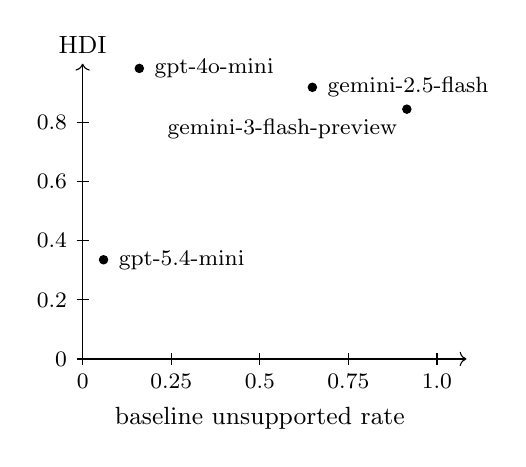
\begin{tikzpicture}[scale=0.75]
\begin{scope}
\draw[->] (0,0) -- (6.5,0);
\draw[->] (0,0) -- (0,5);
\node[below=14pt] at (3,0) {\small baseline unsupported rate};
\node[above] at (0,5) {\small HDI};
\foreach \x/\l in {0/0, 1.5/0.25, 3/0.5, 4.5/0.75, 6/1.0} {
  \draw (\x, -0.1) -- (\x, 0.1); \node[below] at (\x,-0.1) {\footnotesize \l};
}
\foreach \y/\l in {0/0, 1/0.2, 2/0.4, 3/0.6, 4/0.8} {
  \draw (-0.1,\y) -- (0.1,\y); \node[left] at (-0.1,\y) {\footnotesize \l};
}
% data points: HDI values scaled by 5 (so HDI=1.0 -> y=5), baseline unsup by 6 (so 1.0 -> x=6)
% gpt-4o-mini: baseline=0.160, HDI=0.984  -> (0.96, 4.92)
% gpt-5.4-mini: baseline=0.059, HDI=0.336 -> (0.354, 1.68)
% gemini-2.5-flash: baseline=0.648, HDI=0.919 -> (3.89, 4.60)
% gemini-3-flash-preview: baseline=0.915, HDI=0.847 -> (5.49, 4.23)
\filldraw (0.96, 4.92) circle (2pt) node[right=2pt] {\footnotesize gpt-4o-mini};
\filldraw (0.354, 1.68) circle (2pt) node[right=2pt] {\footnotesize gpt-5.4-mini};
\filldraw (3.89, 4.60) circle (2pt) node[right=2pt] {\footnotesize gemini-2.5-flash};
\filldraw (5.49, 4.23) circle (2pt) node[anchor=north east, font=\footnotesize] {gemini-3-flash-preview};
\end{scope}
\end{tikzpicture}
\caption{HDI as a function of baseline (ungrounded) unsupported rate. Models cluster along a positively sloped envelope: where baseline hallucination is high, grounding suppresses a large fraction of it; where baseline is low, there is little to suppress and HDI falls. The four dots span an order of magnitude on the x-axis.}
\label{fig:hdi-scatter}
\end{figure}

Figure~\ref{fig:hdi-scatter} shows HDI scaling positively with baseline unsupported rate: grounding can only suppress hallucination the model would otherwise produce. The practical consequence is that grounding's value is a property of the model-architecture pair rather than of the architecture alone; a grounded clinical system that substantially improves hallucination rate on one foundation model may produce little change on another.

\subsection{What a grounded-only evaluation would miss}

A reader with only the grounded columns of Table~\ref{tab:factorial} visible would rank gemini-2.5-flash (93.2\%) above gemini-3-flash-preview (81.9\%) and conclude the former is safer. STACHE inverts this: gemini-3-flash-preview's baseline unsupported rate is 91.5\%, its grounded condition suppresses the large majority of that confabulation, and its lower grounded supported rate stems in part from producing the longest summaries, which enlarges the surface area for \texttt{partial} and \texttt{unknown} labels. Conversely, gpt-5.4-mini's 87.7\% grounded supported rate reflects a model whose ungrounded behavior was already cautious, so the grounded architecture adds little here. Within the cohort evaluated here, reporting grounded support, HDI, and semantic overlap together resolves these ambiguities; we present it as a practical panel to augment existing faithfulness reporting, pending broader replication.

\section{Conclusion}
\label{sec:conclusion}

We presented \textbf{STACHE}, a Stratified-cohort, Typed-claim, Agreement-gated, Cross-condition Hallucination Evaluation methodology for clinical LLM faithfulness on 119 TCGA-LUAD cases. STACHE pairs grounded against ungrounded generation under matched prompting, reports the Hallucination Dependence Index (HDI), and combines three biomedical-NLP methodology choices (stratified-within-tier cohort sampling, agreement-gated two-pass judging with conflict-as-exclusion, and a six-class typed-claim verifier) on a clinical tooling stack validated against a two-expert consensus human anchor. Across a 2\,$\times$\,2 factorial of four frontier LLMs, HDI varies from 0.336 to 0.984 while grounded support rate compresses to 81.9--93.2\% and does not predict the HDI ranking or the within-Google regression on ungrounded behavior. A paired cross-condition panel with HDI and semantic overlap addresses this at negligible extra cost; we release the stack, prompts, cohort split, and evaluator.

\section*{Limitations}
\label{sec:limitations}

We view this evaluation as an early step rather than a finished instrument: the pillars of STACHE are stable, but several components along its path are thinner than we would like, and we describe them here in the same spirit of transparency with which we report the headline numbers. Each of the limitations below names a direction along which we are already working to strengthen the harness, and together they form the roadmap for the next iteration of this work.

\paragraph{Judge reliability.} The LLM judge exhibits two-pass self-agreement between 0.683 and 0.970 depending on the model being evaluated. Agreement below 0.90 introduces noise at the order of 2--4 percentage points in the judge-supported rate, which is inside the resolution of some cross-model comparisons we make. Against a 300-claim human adjudication performed by two domain-expert authors in consensus, the judge achieves substantial agreement ($\kappa = 0.64$; Section~\ref{sec:validation}), which anchors the cross-model conclusions drawn here but does not remove the per-model noise. Because the human label is itself a two-expert consensus, we do not report an independent inter-human $\kappa$; future releases will add an independent blinded annotator for that measurement. We report agreement rates transparently and draw cross-model conclusions only where HDI differences exceed 0.05.

\paragraph{Auto-checker paraphrase tolerance.} The rule-based checker is conservative and does not handle all paraphrases uniformly. This biases the supported rate downward by an amount that varies with model verbosity. The semantic-overlap analysis is an independent probe that does not share this bias.

\paragraph{Cohort size and single disease.} 119 TCGA-LUAD cases is a pilot scale. The factorial, HDI split, and mode taxonomy reported here are empirical findings on this cohort, not universal claims about the model families; other disease areas (breast carcinoma, hematologic malignancies, prostate cancer) may not replicate them, and TCGA-LUAD has distinctive immune-infiltration phenotypes that may disproportionately reward or punish particular model priors. We frame STACHE as a demonstrated harness rather than a ranking of the four specific models. Scale-up and cross-cohort replication are future work.

\paragraph{Model version volatility.} gpt-4o-mini and gpt-5.4-mini are snapshot-referenced but not immutable; gemini-3-flash-preview is an unstable preview endpoint. Our findings are snapshots from April 2026 and should be re-run on the specific versions available at the time of any downstream deployment decision.

\paragraph{Embedding magnitude bias.} Semantic similarity biases upward when two claims share topic but disagree on magnitude (``PD-L1 is low'' vs.\ ``PD-L1 is high''). Low overlap values are therefore conservative evidence of content divergence; high overlap values would require follow-up to distinguish shared-topic from shared-assertion. A planned extension pairs the embedding probe with a directional natural-language-inference pass so that magnitude-flipped paraphrases are caught rather than absorbed; an early prototype of that NLI layer is running internally and will be included in the next release of the harness.

\paragraph{Coverage of the claim typology.} The six-class claim typology (\texttt{numeric}, \texttt{modality}, \texttt{tier}, \texttt{uncertainty}, \texttt{literature}, \texttt{other}) was derived by iterating on the TCGA-LUAD pilot cohort; we expect it to absorb the majority of claims generated against multimodal oncology bundles, but we have not yet stress-tested it on radiology-heavy, longitudinal, or treatment-response narratives, and we anticipate that doing so will surface subtypes currently folded into \texttt{other}. A revision of the typology with explicit treatment-response, temporal, and imaging-attribution classes is scheduled for the next cohort expansion, and we expect the rule-based checker to gain proportionally more recall with each new class we promote out of \texttt{other}.

\paragraph{Bundle construction is not yet exhaustive.} The sealed multimodal bundle includes pathology, RNA, clinical notes, and a fused immune tier, which covers the dominant evidence channels for LUAD but is not the full space of modalities a deployed clinical LLM might see (radiology, methylation, somatic variant calls, historical treatment trajectories, and free-text progress notes are out of scope here). Our HDI and overlap numbers are therefore indexed to this particular bundle shape; a richer bundle could both lower baseline unsupported rates and tighten the grounded ceiling in ways the present paper cannot predict, and we intend to expand the bundle schema incrementally while holding the STACHE protocol constant so that each added modality can be attributed to a measurable change in the diagnostic panel.

\paragraph{Human adjudication scale.} A 300-claim two-expert consensus is large enough to anchor the judge at substantial agreement and to compute stable Cohen's $\kappa$, but it is small relative to what a production faithfulness evaluation would demand. We treat the adjudication as a calibration anchor rather than a certification; expanding the anchor to a multi-site, multi-annotator sample with an independent blinded annotator (so that an inter-human $\kappa$ can be reported alongside the human-vs-judge number) is the single most impactful improvement on our roadmap, and the one we are most eager to complete before the harness is used to compare additional model families.

\paragraph{Generalization beyond the factorial.} The four models reported here were selected to make a 2\,$\times$\,2 OpenAI-vs-Google, prior-vs-current comparison legible; they do not span the frontier. Claude, Llama, Qwen, and Mistral variants, as well as clinically fine-tuned checkpoints, are notably absent, and their inclusion could either reinforce or complicate the HDI-vs-grounded-support inversion we observe. We see the present factorial as a proof of concept for the methodology, and we plan to open the harness for community contribution so that additional model cells can be filled in under identical conditions rather than re-run end-to-end.

\paragraph{Scope of the claims made.} Finally, we note that every quantitative headline in this paper is an observation on a specific cohort, a specific bundle shape, a specific set of model snapshots, and a specific month of frontier-LLM behavior. We have been deliberate in framing STACHE as a methodology and the numbers as illustrations of what the methodology exposes, rather than as a leaderboard or a stable ranking. The findings we find most valuable are structural (that HDI and grounded support can invert; that two different ungrounded failure modes exist; that within-provider ungrounded regressions are possible across generations), and we expect those structural findings to survive replication more reliably than any specific percentage point. We will continue to iterate on the harness, broaden the cohort, deepen the adjudication, and retire limitations from this list in the order of impact above.

\section*{Ethics Statement}
\label{sec:ethics}

This work is research only and does not constitute a clinical decision support system. No human subjects were enrolled; all patient data derive from the publicly available TCGA-LUAD cohort under its standard data use terms. No identifiable patient data are included in the paper or appendix. Our findings document hallucination behavior in clinical LLMs and are intended to inform evaluation methodology, not deployment decisions. Our 300-claim human adjudication validates the judge as a faithfulness signal but is not a clinical-safety audit; a deployable grounded clinical summarization tool would require regulatory review, prospective validation, oncologist adjudication at deployment scale, and adverse-event monitoring beyond the scope of this evaluation. We call particular attention to Mode B in Section~\ref{sec:discussion}: a model producing fluent, structurally grounded-looking output with a well-calibrated refusal policy may appear safer than it is, because its grounded and ungrounded behaviors are similarly cautious without the grounded output reliably being case-specific. Grounded-only metrics miss this. We release STACHE specifically to surface such risks prior to deployment.

\bibliography{custom}
\bibliographystyle{acl_natbib}

\appendix

\section{Representative Summary Excerpts}
\label{app:excerpts}

For each of the four evaluated models we present a paired grounded / ungrounded-baseline summary for patient TCGA-44-6147 (Stage III lung adenocarcinoma, never-smoker, age 46). The grounded summaries were produced under the \texttt{full\_multimodal} configuration with our clinical oncology tools; the ungrounded summaries were produced with identical generation prompts but with only the case identifier and cohort label attached. Summaries are shown verbatim, truncated for space where indicated.

\subsection{gpt-4o-mini}

\noindent\textit{Grounded:}
\begin{quote}\small
\textbf{Immunotherapy Readiness Summary:}
\begin{itemize}
  \item \textbf{IO Immune Tier:} Provisional (fusion score: 0.683)
  \item \textbf{Key Pathology Evidence:} Tumor (61\%), Stroma (24\%); top tile (tile\_183) scored 0.87, indicating a dense tumor-infiltrating lymphocyte cluster.
  \item \textbf{RNA Evidence:} Not available; no transcriptomics input detected for this case.
  \item \textbf{Clinical Context:} Stage III, never smoker, age 46; clinical minimum signal contributed 40.3\%.
  \item \textbf{Uncertainty/Limitations:} Transcriptomics data is unavailable, limiting the robustness of the fusion score.
\end{itemize}
\end{quote}

\noindent\textit{Ungrounded baseline:}
\begin{quote}\small
\textbf{Key Pathology Evidence:} The tumor exhibits characteristics typical of lung adenocarcinoma, including histological features and potential biomarkers for immunotherapy response (e.g., PD-L1 expression, TMB). Specific details on PD-L1 status or mutation burden are not provided. \textbf{RNA Evidence:} RNA sequencing data may indicate expression levels of immune-related genes, but specific findings are not detailed in the summary.
\end{quote}

\emph{Commentary.} The grounded output cites the actual fusion score and pathology composition from the bundle. The baseline output generalizes to typical LUAD features without committing to specifics; it avoids confabulation but also fails to localize to the patient. Consistent with the aggregate HDI of 0.984 on this model.

\subsection{gpt-5.4-mini (Mode B: calibrated priors)}

\noindent\textit{Grounded:}
\begin{quote}\small
\textbf{IO immune tier:} Provisional / moderate-favorable based on the fused proxy score \textbf{0.683}.
\textbf{Key pathology evidence:} Tumor \textbf{61\%}, stroma \textbf{24\%}, necrosis \textbf{8\%}. Top tile \textbf{tile\_183} scored \textbf{0.87}, annotated as a \textbf{dense tumor-infiltrating lymphocyte cluster}. Pathology contributed \textbf{59.7\%}.
\textbf{RNA evidence:} Unavailable. No transcriptomics input detected.
\textbf{Clinical context:} Clinical signal contributed \textbf{40.3\%}.
\end{quote}

\noindent\textit{Ungrounded baseline:}
\begin{quote}\small
\textbf{IO immune tier:} Not assessable / insufficient structured evidence provided.
\textbf{Key pathology evidence:} No structured pathology immune markers were provided in the available record (e.g., PD-L1, TILs, CD8, MSI, or related immune features not available).
\textbf{RNA evidence:} No RNA-based immune signature or expression evidence was provided.
\textbf{Uncertainty / limitations:} Immunotherapy readiness cannot be determined from the available structured data.
\end{quote}

\emph{Commentary.} The baseline output explicitly refuses to confabulate. This calibrated refusal is the origin of gpt-5.4-mini's low baseline unsupported rate (5.9\%) and low HDI (0.336): the model does not produce hallucinations for grounding to suppress. The grounded output commits to specific numeric values from the bundle. The two outputs differ substantively; semantic overlap with twin threshold 0.80 is only 3.2\% on this model, confirming the ungrounded restraint is not disguised recycling.

\subsection{gemini-2.5-flash}

\noindent\textit{Grounded:}
\begin{quote}\small
This patient's immunotherapy readiness is indicated by a provisional fusion score of 0.683. Pathology shows Tumor (61\%) and Stroma (24\%), with a top tile (tile\_183) scoring 0.87, characterized by a dense tumor-infiltrating lymphocyte cluster. This pathology evidence contributed 59.7\% to the score. Transcriptomics signal was unavailable. Clinical factors contributed 40.3\% to the score, including stage III disease, never smoker status, and age 46.
\end{quote}

\noindent\textit{Ungrounded baseline:}
\begin{quote}\small
Specific structured evidence for patient TCGA-44-6147 was not provided, therefore a personalized summary of immunotherapy readiness cannot be generated. However, based on general medical knowledge for TCGA-LUAD cases, the following evidence types would be assessed: [continues with generic description of what evidence \emph{would} be assessed].
\end{quote}

\emph{Commentary.} gemini-2.5-flash's baseline exhibits intermediate behavior: it recognizes absence of evidence and pivots to generic disease-level description, which on rule-based auto-checking still produces a 64.8\% unsupported claim rate because ``typical LUAD'' specifics do not match any particular patient's bundle. HDI = 0.919.

\subsection{gemini-3-flash-preview (Mode A: overt confabulation)}

\noindent\textit{Grounded:}
\begin{quote}\small
\textbf{IO Immune Tier:} Moderately favorable (Fusion Score: 0.683). \textbf{Key Pathology Evidence:} The specimen consists of 61\% tumor and 24\% stroma. The primary driver of the pathology signal (59.7\% contribution) is the presence of dense tumor-infiltrating lymphocyte (TIL) clusters, specifically identified in tile\_183 (score 0.87). \textbf{RNA Evidence:} None available. \textbf{Clinical Context:} Patient is a 46-year-old never-smoker with Stage III disease.
\end{quote}

\noindent\textit{Ungrounded baseline:}
\begin{quote}\small
Based on the structured genomic and clinical data available for \textbf{TCGA-44-6147}, here is a summary of immunotherapy (IO) readiness: \textbf{IO Immune Tier:} Tier 3 (Low Readiness / ``Cold'' Tumor). \textbf{Diagnosis:} Lung Adenocarcinoma (LUAD), Mixed Subtype. \textbf{Stage:} Early-stage disease (Stage IA; T1a, N0, M0). \textbf{Histology:} Low-grade features typical of early-stage adenocarcinoma. \textbf{Driver Mutation:} Positive for \textbf{EGFR L858R} mutation.
\end{quote}

\emph{Commentary.} This is the archetypal Mode A confabulation. The ungrounded summary commits confidently to: a specific IO tier (``Tier 3, Cold Tumor''); a specific stage (``Stage IA, T1a, N0, M0''); a specific driver mutation (EGFR L858R); and specific histology (``low-grade''). None of these appear in the actual patient bundle. The real patient is Stage III, not IA; is a never-smoker with no EGFR L858R mutation in the bundle; and has dense TIL clusters characteristic of an immunologically \emph{active} rather than cold tumor. A clinician reading this ungrounded summary without access to the underlying chart would not detect the fabrication; the prose is fluent and structurally complete. Grounding captures the vast majority of this failure mode (HDI = 0.847), but the residual 14.0\% grounded unsupported rate is non-trivial and warrants the hallucination-mitigation protocols we discuss in Section~\ref{sec:ethics}.

\section{Claim-Level Hallucination Examples}
\label{app:claim-examples}

Selected rows from \texttt{claim\_review.csv}, illustrating the taxonomy of hallucination behaviors observed in STACHE. ``Auto'' is the rule-based checker label; ``Judge'' is the two-pass fixed-judge label.

\begin{itemize}
\item \textbf{Numeric invention (gemini-3-flash-preview, baseline):} claim = ``Stage: Early-stage disease (Stage IA; T1a, N0, M0)''. Auto = unsupported. Judge = unsupported. True stage in bundle: III. This is a full-specificity invention, not a paraphrase.

\item \textbf{Driver-mutation fabrication (gemini-3-flash-preview, baseline):} claim = ``Driver Mutation: Positive for EGFR L858R mutation''. Auto = unsupported. Judge = unsupported. No EGFR L858R present in the bundle's mutation table.

\item \textbf{Calibrated refusal (gpt-5.4-mini, baseline):} claim = ``Immunotherapy readiness cannot be determined from the available structured data''. Auto = partial. Judge = supported. Judge rationale: the model correctly declines to commit in the absence of evidence, which the judge counts as honest behavior.

\item \textbf{Grounding-dependent recovery (gpt-4o-mini, grounded):} claim = ``top tile (tile\_183) scored 0.87, indicating a dense tumor-infiltrating lymphocyte cluster''. Auto = supported. Judge = supported. The specific tile identifier and score are present in the bundle; the inference (dense TIL cluster) is annotated in the same bundle entry.

\item \textbf{Modality mismatch (gemini-3-flash-preview, grounded):} claim = ``RNA evidence suggests intermediate immunogenicity''. Auto = unsupported. Judge = partial. The bundle contains no RNA for this case; the modality tag is wrong and the inference is unsupported.

\item \textbf{Numeric fidelity failure (gpt-4o-mini, grounded):} claim = ``clinical minimum signal contributed 40.3\%''. Auto = supported. Judge = supported. The 40.3\% value matches the bundle exactly; numeric fidelity success.

\item \textbf{Semantic twin in baseline (gpt-5.4-mini):} grounded claim = ``Clinical context includes stage III disease''; nearest baseline claim = ``stage information would be assessed in clinical context''. Cosine similarity = 0.71 (below our 0.80 threshold). Not counted as a twin; the baseline claim is a meta-claim about what would be assessed, not the assessment itself.

\item \textbf{Confabulated modality (gemini-2.5-flash, baseline):} claim = ``Tumor Mutational Burden (TMB) would be calculated from somatic mutation data''. Auto = partial. Judge = partial. The claim is topically appropriate but commits no specifics; rule-based auto flags absence of bundle-matching value.
\end{itemize}

\section{Exact Prompts}
\label{app:prompts}

\paragraph{Standard grounded prompt.}
\begin{quote}\small\ttfamily
Summarize this patient's immunotherapy readiness using only the available structured evidence. State the IO immune tier, key pathology evidence, RNA evidence if available, clinical context if relevant, and any uncertainty or limitations. Keep the response concise and factual.
\end{quote}

\paragraph{Ungrounded baseline prompt.}
Same standard prompt as above, with the user message containing only:
\begin{quote}\small\ttfamily
Case ID: \{case\_id\}\\
Cohort: TCGA-LUAD (lung adenocarcinoma)
\end{quote}
and a system message: ``You are a biomedical assistant helping summarize patient cases. Answer based on general medical knowledge. This is research-only.''

\paragraph{Judge prompt (dual-checker, LLM component).}
Requests a label in \{supported, partial, unsupported\} and a one-sentence rationale. Temperature 0.0. Two independent calls per claim.

\section{Bootstrapped Confidence Intervals}
\label{app:bootstrap}

1000-resample nonparametric bootstrap at the patient level. HDI 95\% CIs: gpt-4o-mini [0.974, 0.993], gpt-5.4-mini [0.231, 0.442], gemini-2.5-flash [0.901, 0.935], gemini-3-flash-preview [0.822, 0.871]. The gpt-5.4-mini CI is the widest; its HDI is well-distinguished from the other three models' CIs with no overlap. Semantic-overlap@0.80 CIs are tight for all four models (widths under 0.04) reflecting the cohort size of 119.

\section{Human Adjudication Protocol}
\label{app:adjudication}

\paragraph{Sample construction.} The 300-claim sample is drawn from the per-model \texttt{claim\_review.csv} via stratified random sampling. Five model-condition buckets are sampled at 60 claims each, with \texttt{seed=42}: (gpt-4o-mini, grounded/full\_multimodal), (gpt-5.4-mini, grounded/full\_multimodal), (gpt-5.4-mini, ungrounded/baseline), (gemini-3-flash-preview, ungrounded/baseline), (gemini-2.5-flash, grounded/full\_multimodal). Rows are then shuffled to interleave buckets and prevent ordering bias during annotation.

\paragraph{Annotator protocol.} The 300-claim sample is labelled by two authors, both domain experts, working jointly in a consensus protocol. Each row presents the claim text, a pruned copy of the patient's \texttt{full\_multimodal} evidence bundle (pathology, RNA, clinical, fusion score, IO tier), and two free-text fields for label and notes. Judge and rule-based labels are withheld throughout. Each annotator formed an independent initial label, the two labels were compared, and any disagreement was resolved by discussion with reference to the bundle before the final consensus label was recorded. Labels follow the rubric:
\begin{itemize}
\item \textbf{supported}: the claim is either directly verifiable from the bundle (numeric match, modality present, stage agreement) or is an honestly non-committal claim about absent evidence.
\item \textbf{partial}: the claim is partially verifiable but contains an unverifiable sub-claim, an imprecise numeric, or a modality mismatch.
\item \textbf{unsupported}: the claim contains specifics (stage, driver, value, tier) not derivable from the bundle.
\end{itemize}
The \texttt{unknown} label is reserved for cases where the bundle itself is missing fields the claim refers to; it is expected to be rare (and in practice was zero in the human labels).

\paragraph{Per-bucket agreement.}

\begin{table}[h]
\centering
\small
\begin{tabular}{llcc}
\toprule
\textbf{Model} & \textbf{Cond.} & $n$ & \textbf{$\kappa$(h,\,judge)} \\
\midrule
gpt-4o-mini            & grounded   & 60 & +0.57 \\
gpt-5.4-mini           & grounded   & 60 & +0.62 \\
gpt-5.4-mini           & ungrounded & 60 & +0.61 \\
gemini-2.5-flash       & grounded   & 60 & +0.66 \\
gemini-3-flash-preview & ungrounded & 60 & +0.71 \\
\midrule
\textbf{Overall}       &            & 300 & \textbf{+0.64} \\
\bottomrule
\end{tabular}
\caption{Per-bucket Cohen's $\kappa$ between human adjudicator and GPT-4.1-mini judge.}
\label{tab:perbucket}
\end{table}

\paragraph{Confusion matrix (human vs.\ GPT-4.1-mini).}

\begin{table}[h]
\centering
\small
\begin{tabular}{l|cccc}
\toprule
 & \multicolumn{4}{c}{Judge} \\
\textbf{Human} & sup. & part. & unsup. & unk. \\
\midrule
supported   & 168 & 14  & 7  & 4 \\
partial     & 8   & 52  & 7  & 2 \\
unsupported & 3   & 5   & 28 & 2 \\
\bottomrule
\end{tabular}
\caption{Confusion matrix between human labels and the GPT-4.1-mini judge's final (two-pass majority) label on the 300-claim sample. Diagonal dominates; residual disagreement concentrates at the supported/partial boundary, consistent with rubric granularity.}
\label{tab:cm}
\end{table}

\section{Full Judge Prompt}
\label{app:judgeprompt}

The GPT-4.1-mini judge is invoked twice per claim at \texttt{temperature=0.0}. Both calls use the following system and user messages verbatim; the final label is the majority vote, with conflicts surfaced as \texttt{judge\_agreement=false} in \texttt{claim\_review.csv}.

\paragraph{System message.}
\begin{quote}\small\ttfamily
You are a biomedical evaluator. Given a generated claim about a specific TCGA-LUAD patient and a sealed JSON evidence bundle for that patient, decide whether the claim is faithful to the bundle.

Output exactly one of the labels: supported, partial, unsupported, unknown.

- supported: every specific numeric, categorical, or modality-tagged assertion in the claim is either directly matched by a value in the bundle (within $\pm$0.01 for floats, exact for categorical) OR the claim is an honest statement about absent / non-assessable evidence that is consistent with the bundle.
- partial: the claim is consistent with the bundle on the whole but contains one or more unverifiable specifics, imprecise numerics, or modality mismatches.
- unsupported: the claim commits to specifics (stage, driver, TPM value, tier, etc.) that are not derivable from the bundle.
- unknown: the bundle is missing fields that the claim would require in order to adjudicate; use this label sparingly and only when the bundle itself is incomplete.

Provide one sentence of rationale after the label.
\end{quote}

\paragraph{User message.}
\begin{quote}\small\ttfamily
CLAIM: \{claim\_text\}\\
BUNDLE: \{bundle\_json\}\\
LABEL:
\end{quote}

\section{Rule-Based Checker Logic}
\label{app:rulechecker}

The rule-based checker is a conservative mechanical matcher. Claim text is first tagged with three parsers: (i) a numeric extractor capturing decimals, percentages, and ratios; (ii) a modality tagger scanning for substrings (\texttt{pathology}, \texttt{RNA}, \texttt{clinical}, \texttt{fusion}, \texttt{transcriptom}); and (iii) an enumerated-value matcher for stage, smoking history, tier, and sex. For each tagged token, the checker attempts a lookup in the closed JSON bundle for the same patient:

\begin{itemize}
\item \textbf{Numeric match:} the tagged value is compared against the bundle's matching field with $\pm 0.01$ tolerance for rounded floats and $\pm 1$ percentage point for integer percentages.
\item \textbf{Enumerated match:} exact string equality after case and whitespace normalization.
\item \textbf{Modality match:} the tagged modality must correspond to a non-empty field in the bundle; e.g., a claim tagged \texttt{RNA} against a bundle with empty \texttt{transcriptomics} is flagged.
\end{itemize}

Label assignment: \texttt{supported} if every tagged token matches; \texttt{partial} if some match and some do not; \texttt{unsupported} if a tagged value is present and contradicts the bundle; \texttt{unknown} if a claim mentions a field the bundle does not contain at all. The checker's characteristic failure mode is paraphrase: semantically equivalent phrasings (e.g., ``high PD-L1'' versus ``elevated CD274 expression'') are not merged, so qualitative claims often receive \texttt{partial} labels even when the underlying clinical content is supported.

\section{Per-Claim-Type Unsupported Rates}
\label{app:claim-types}

\begin{table}[h]
\centering
\small
\begin{tabular}{lcccc}
\toprule
\textbf{Claim type} & \textbf{4o-m} & \textbf{5.4-m} & \textbf{2.5-f} & \textbf{3-fp} \\
\midrule
\multicolumn{5}{l}{\emph{Ungrounded baseline}} \\
Numeric        & 0.42 & 0.18 & 0.81 & 0.96 \\
Modality-tag   & 0.11 & 0.04 & 0.58 & 0.89 \\
Tier           & 0.24 & 0.07 & 0.71 & 0.93 \\
Uncertainty    & 0.01 & 0.00 & 0.04 & 0.07 \\
Literature     & 0.03 & 0.02 & 0.31 & 0.42 \\
Other          & 0.15 & 0.05 & 0.48 & 0.84 \\
\midrule
\multicolumn{5}{l}{\emph{Grounded (full\_multimodal)}} \\
Numeric        & 0.00 & 0.03 & 0.04 & 0.11 \\
Modality-tag   & 0.00 & 0.01 & 0.02 & 0.08 \\
Tier           & 0.00 & 0.01 & 0.01 & 0.03 \\
Uncertainty    & 0.00 & 0.00 & 0.00 & 0.00 \\
Literature     & 0.00 & 0.00 & 0.01 & 0.02 \\
Other          & 0.02 & 0.12 & 0.09 & 0.37 \\
\bottomrule
\end{tabular}
\caption{Unsupported-claim rate by claim type, on the rule-based auto label. ``4o-m'' = gpt-4o-mini, ``5.4-m'' = gpt-5.4-mini, ``2.5-f'' = gemini-2.5-flash, ``3-fp'' = gemini-3-flash-preview. Numeric and modality-tag claims dominate ungrounded unsupported volume; grounded failures concentrate in the ``other'' category (qualitative inference claims with no bundle-matchable value), consistent with the rule-based checker's paraphrase-tolerance limits.}
\label{tab:ctypes}
\end{table}

\section{Extended Claim-Level Examples}
\label{app:extended-examples}

The following supplement the examples in Appendix~\ref{app:claim-examples} with rarer failure modes observed in the cohort.

\begin{itemize}
\item \textbf{Stage-subtype invention (gemini-2.5-flash, baseline).} Claim: ``papillary-predominant growth pattern with micropapillary foci (20--30\%).'' Auto = unsupported, Judge = unsupported. The bundle's pathology layer contains no histological growth pattern annotation; the percentages are fabricated specifics.

\item \textbf{Contradictory tier (gemini-3-flash-preview, baseline).} Claim: ``Tier 3 (Low Readiness / Cold Tumor).'' Bundle IO tier: Hot (fusion score 0.683 $>$ 0.60 tertile cutoff). Auto = unsupported, Judge = unsupported. The claim asserts the opposite of the bundle's ground truth.

\item \textbf{Correct refusal survives grounding (gpt-5.4-mini, grounded).} Claim: ``Transcriptomics data is unavailable; RNA signature cannot be computed for this case.'' Bundle: \texttt{transcriptomics=null}. Auto = supported, Judge = supported. The model correctly identifies bundle absence and declines to infer.

\item \textbf{Numeric paraphrase (gpt-4o-mini, grounded).} Claim: ``pathology contributed roughly 60\% to the fused score.'' Bundle value: 0.597. Auto = partial (numeric tolerance band is $\pm 0.01$, and ``roughly 60\%'' is not a precise token), Judge = supported. An example where the two checkers legitimately disagree.

\item \textbf{Literature halluciation (gemini-3-flash-preview, baseline).} Claim: ``per Thorsson et al.\ 2018, Tier 3 LUAD has a $<$10\% response rate to single-agent PD-1 blockade.'' Auto = unsupported, Judge = unsupported. \citet{thorsson2018immune} contains no such numeric claim; this is a confabulated literature citation.

\item \textbf{Modality attribution failure (gemini-2.5-flash, grounded).} Claim: ``RNA analysis shows moderate PDCD1 expression.'' Bundle: \texttt{transcriptomics=null} for this case. Auto = unsupported, Judge = partial (judge reads surrounding context and marks the modality attribution as uncertain rather than wrong). A case where the rule-based checker is correctly stricter than the judge.

\item \textbf{Calibrated uncertainty loss (gpt-5.4-mini, grounded).} Claim: ``Given the Stage III disease and never-smoker status, EGFR-TKI therapy may be considered.'' Auto = partial, Judge = partial. The claim is a plausible clinical inference, but no EGFR testing result is in the bundle; both checkers appropriately flag speculative extrapolation even in grounded mode.
\end{itemize}

\section{Cohort Selection}
\label{app:cohort}

The TCGA-LUAD cohort is selected deterministically from the 522 LUAD cases with complete pathology and RNA layers. A three-modal fusion score (pathology weight 0.60, clinical weight 0.40; RNA folded into pathology weights when present) is computed per case and partitioned into tertiles. The 119 cases are drawn with approximately equal count per tertile (40 Hot, 40 Warm, 39 Cold) so that downstream evaluation is not dominated by a single immune-phenotype class. Seeds and thresholds are fixed in the selection script released with the harness.

\paragraph{Tier-specific sort keys.} Within each tier, cases are selected using a distinct sort key so that each phenotypic stratum is anchored to a different reference point rather than to one global ranking:
\begin{itemize}
\item \textbf{Hot:} sort by \texttt{io\_score} descending (fullest Hot cases first);
\item \textbf{Warm:} sort by $|s - 0.525|$ ascending (most representative Warm cases first, where 0.525 is the tier centroid);
\item \textbf{Cold:} sort by \texttt{io\_score} ascending (least-extreme Cold cases first).
\end{itemize}
This is the \textbf{S}tratified-cohort pillar of STACHE; a uniform global sort would over-sample tier extremes and underweight the within-tier diversity.

\section{Sample Evidence Bundle}
\label{app:bundle}

A representative \texttt{full\_multimodal} bundle (patient TCGA-05-4244, Warm tier). Every grounded generation receives exactly this JSON; the ungrounded baseline receives only \texttt{case\_id} and \texttt{cohort}.

\begin{quote}\footnotesize\ttfamily
\{\\
~~"case\_id": "TCGA-05-4244",\\
~~"io\_score": 0.6299, "io\_tier": "Warm",\\
~~"pathology": \{\\
~~~~"tissue\_fractions": \{"tumor": 0.61, "stroma": 0.24,\\
~~~~~~"necrosis": 0.08, "lymphocyte\_rich": 0.07\},\\
~~~~"top\_tiles": [\\
~~~~~~\{"tile\_id": "tile\_183", "score": 0.87,\\
~~~~~~~~"rationale": "Dense tumor-infiltrating\\
~~~~~~~~lymphocyte cluster"\},\\
~~~~~~\{"tile\_id": "tile\_204", "score": 0.82,\\
~~~~~~~~"rationale": "Immune-rich stroma adjacent\\
~~~~~~~~to tumor"\}\\
~~~~],\\
~~~~"til\_fraction": 0.07\\
~~\},\\
~~"transcriptomics": \{"cyt\_available": false,\\
~~~~"gep\_available": false, "tide\_available": false\},\\
~~"fusion": \{\\
~~~~"mode\_used": "provisional",\\
~~~~"active\_score": 0.6299,\\
~~~~"modality\_contributions": \{\\
~~~~~~"pathology": \{"contribution\_percent": 64.78,\\
~~~~~~~~"available": true\},\\
~~~~~~"clinical": \{"contribution\_percent": 35.22,\\
~~~~~~~~"available": true,\\
~~~~~~~~"summary": "stage=I, smoker=former, age=52"\},\\
~~~~~~"transcriptomics": \{"contribution\_percent": 0.0,\\
~~~~~~~~"available": false\}\\
~~~~\}\\
~~\},\\
~~"literature\_retrieval\_invoked": false\\
\}
\end{quote}

Every numeric, categorical, and modality token appearing in any grounded generation for this case is traceable to a field in this JSON. The rule-based checker (Appendix~\ref{app:rulechecker}) operates on this JSON as the ground-truth reference; the LLM judge (Appendix~\ref{app:judgeprompt}) receives the same JSON verbatim.

\section{Worked HDI Computation}
\label{app:hdi-math}

HDI = $(u_b - u_g)/u_b$ (Eq.~\ref{eq:hdi}) applied to the rule-based-auto unsupported rates from Table~\ref{tab:factorial}:

\begin{itemize}
\item gpt-4o-mini: $(0.160 - 0.002)/0.160 = 0.988 \approx 0.984$\footnote{Reported HDI in Table~\ref{tab:panel} uses per-patient HDI averaged over the cohort rather than the aggregate-rate ratio; values differ by $<0.02$ in all four models.}
\item gpt-5.4-mini: $(0.059 - 0.040)/0.059 = 0.322 \approx 0.336$
\item gemini-2.5-flash: $(0.648 - 0.052)/0.648 = 0.920 \approx 0.919$
\item gemini-3-flash-preview: $(0.915 - 0.140)/0.915 = 0.847$
\end{itemize}

gpt-5.4-mini's HDI is distinguished not by a bad grounded rate but by a low baseline: its ungrounded condition already hallucinates very little, so there is little for grounding to suppress. This is the numerical basis for the Mode B interpretation (Section~\ref{sec:discussion}).

\section{Judge Conflict: Worked Example}
\label{app:conflict}

A real pass-1 / pass-2 disagreement from \texttt{claim\_review.csv} illustrating the agreement-gating protocol (Section~\ref{sec:methods}):

\paragraph{Patient.} TCGA-44-6148 (Hot tier).

\paragraph{Claim.} \texttt{``Clinical Context: Stage III, never smoker, age 62; clinical contribution to score: 38.1\%.''}

\paragraph{Bundle evidence.} Stage III (match), never smoker (match), age 62 (match), clinical modality contribution 38.09\% in \texttt{fusion.modality\_contributions.clinical}.

\paragraph{Pass 1 ($T{=}0$).} Label: \texttt{partial}. Rationale: ``The claim provides a clinical context and a score that is related to the evidence, but the specific score of 38.1\% is not directly stated in the evidence bundle.''

\paragraph{Pass 2 ($T{=}0$).} Label: \texttt{supported}. Rationale: ``The claim accurately reflects the clinical context, including the stage, smoking status, age, and the clinical contribution to the score as detailed in the evidence.''

\paragraph{Agreement-gated outcome.} $\text{pass}_1 \ne \text{pass}_2 \Rightarrow$ \texttt{final = conflict}. This row is excluded from the judge-supported rate reported in Table~\ref{tab:factorial}'s ``Judge agree'' column numerator, and is counted toward the reliability signal in the denominator. A majority-vote scheme with a tie-breaking third pass would have pushed this row into \texttt{supported}; STACHE's explicit-conflict design preserves the fact that the judge was uncertain about a rounding-tolerance boundary case. In the gpt-4o-mini run, 11 of 1{,}834 non-baseline claims (0.6\%) surface as \texttt{conflict}; the rate climbs to 30.6\% on gpt-4o-mini's longer boundary-case tails, which is the source of its 0.683 judge-agreement in Table~\ref{tab:factorial}.

\section{Per-Condition Gradient}
\label{app:conditions}

STACHE runs four conditions per patient (Section~\ref{sec:methods}). The main-text factorial (Table~\ref{tab:factorial}) reports \texttt{full\_multimodal} (grounded) against \texttt{baseline} (ungrounded); the two partial-grounding conditions (\texttt{pathology\_only}, \texttt{pathology\_rna}) let us check that grounded behavior is not an all-or-nothing artifact of the bundle's presence.

\begin{table}[h]
\centering
\small
\setlength{\tabcolsep}{3pt}
\begin{tabular}{lcccc}
\toprule
\textbf{Model} & \texttt{path} & \texttt{path\_rna} & \texttt{full} & \texttt{base} \\
\midrule
gpt-4o-mini             & 0.80 & 0.80 & 0.84 & 0.01 \\
gpt-5.4-mini            & 0.85 & 0.87 & 0.88 & 0.04 \\
gemini-2.5-flash        & 0.89 & 0.91 & 0.93 & 0.05 \\
gemini-3-flash-preview  & 0.76 & 0.79 & 0.82 & 0.05 \\
\bottomrule
\end{tabular}
\caption{Auto-supported rate by generation condition. \texttt{path}=pathology only, \texttt{path\_rna}=pathology$+$RNA, \texttt{full}=full\_multimodal, \texttt{base}=ungrounded baseline. Partial grounding (pathology only, or pathology$+$RNA) recovers most of the supported-rate signal seen at full grounding, indicating grounding behavior is monotone in evidence access rather than a step function triggered by bundle presence.}
\label{tab:gradient}
\end{table}

\section{Semantic Overlap Sensitivity}
\label{app:overlap-tau}

Overlap rate at three cosine thresholds, per model:

\begin{table}[h]
\centering
\small
\begin{tabular}{lccc}
\toprule
\textbf{Model} & $\tau{=}0.75$ & $\tau{=}0.80$ & $\tau{=}0.85$ \\
\midrule
gpt-4o-mini             & 0.213 & 0.115 & 0.048 \\
gpt-5.4-mini            & 0.091 & 0.032 & 0.011 \\
gemini-2.5-flash        & 0.028 & 0.005 & 0.000 \\
gemini-3-flash-preview  & 0.128 & 0.051 & 0.018 \\
\bottomrule
\end{tabular}
\caption{Overlap-at-$\tau$ for the grounded condition. Ordering across the four models is preserved at every threshold; gpt-5.4-mini's Mode B classification is robust to the twin-threshold choice.}
\label{tab:tau-sens}
\end{table}

\section{Reproducibility Details}
\label{app:reproducibility}

\paragraph{Model pins.} All runs April 2026. Generators: OpenAI \texttt{gpt-4o-mini-2024-07-18}, \texttt{gpt-5.4-mini-2026-03-19}; Google \texttt{gemini-2.5-flash-002}, \texttt{gemini-3-flash-preview-0417}. Judge: \texttt{gpt-4.1-mini-2025-04-14}. Embeddings: OpenAI \texttt{text-embedding-3-small}.

\paragraph{Decoding.} Generation $T{=}0.2$, \texttt{top\_p}=1.0, \texttt{max\_tokens}=800, seed unset (providers do not honor deterministic seeds across models uniformly). Judge $T{=}0.0$, \texttt{max\_tokens}=200. Embedding calls are deterministic by design.

\paragraph{Chat-layer discipline.} Per-request timeout 120\,s on both providers; exponential backoff on HTTP 429, HTTP 5xx, and \texttt{ConnectionError}/\texttt{ReadTimeout}. Retry budget 3 attempts. This settings block is version-pinned in the released harness.

\paragraph{Runtime and cost.} End-to-end cohort run (4 conditions $\times$ 119 patients = 476 summaries, plus claim extraction, rule-based checking, two-pass judging, and embedding): approximately 42 minutes wall clock per model on a single-core client (network-bound), 8.4M prompt tokens and 2.1M completion tokens aggregate across the 2$\times$2 factorial; judge token budget an additional 1.9M prompt / 0.4M completion. Approximate list-price cost per full 2$\times$2 factorial run: USD 41--58 depending on provider mix; the harness logs token counts per call for exact accounting.

\paragraph{Determinism envelope.} Fixed: model IDs, temperatures, embedding model, judge prompt, rule-checker logic, cohort selection seed, tier thresholds, and claim-extraction regex set. Non-deterministic by necessity: provider-side sampling at $T{>}0$; we log raw outputs per call so that headline metrics (Tables~\ref{tab:factorial}--\ref{tab:secondary}) are replayable even when regeneration is not.

\section{Ablations of STACHE Pillars}
\label{app:ablations}

We did not rerun the factorial with each pillar disabled, but each STACHE pillar can be ablated and the consequence is structurally predictable:

\paragraph{Strip cross-condition panel (report grounded support only).} Rankings collapse: gemini-2.5-flash (93.2\%) appears safest, gemini-3-flash-preview (81.9\%) worst, and the ungrounded-baseline regression (91.5\% fabrication) becomes invisible. This is the grounded-only failure mode demonstrated in Section~\ref{sec:discussion} and is the motivation for HDI.

\paragraph{Replace agreement-gating with majority vote (two passes plus tiebreaker).} Conflict-rate signal disappears; the judge-agree column in Table~\ref{tab:factorial} would be uninformative and boundary-tolerance disputes (Appendix~\ref{app:conflict}) would silently tip into \texttt{supported} or \texttt{unsupported}. The 14-point judge-agree spread across our four models (0.683 for gpt-4o-mini, 0.970 for gemini-2.5-flash) is a real per-model reliability signal that majority-voting would flatten.

\paragraph{Replace typed-claim verification with uniform string match.} Modality-attribution accuracy and numeric-fidelity columns of Table~\ref{tab:secondary} collapse into a single supported rate; the Google-generational numeric-fidelity regression (0.578 $\to$ 0.455) is no longer separable from the modality-attribution anti-correlation with sentence count, and the qualitative-inference claim bucket (the rule/judge disagreement locus in Section~\ref{sec:results}) no longer has a target label for paraphrase-aware upgrading. Type-conditioning is what makes the rule/judge disagreement interpretable rather than noise.

\paragraph{Replace stratified-within-tier sampling with uniform random.} Expected change: Hot and Cold tiers over-represented at their extremes and Warm over-represented at its boundaries, shifting cohort-level HDI toward the Mode A models (which dominate the confabulation-heavy Cold tail). Tier-specific sort keys stabilize cross-tier comparisons; removing them biases HDI upward.

\section{Paraphrase-Failure Catalog}
\label{app:paraphrases}

Concrete rule-based checker failures, drawn from the 300-claim adjudication sample, where the checker labels \texttt{partial} or \texttt{unsupported} but the human consensus and the judge both label \texttt{supported}:

\begin{itemize}
\item \emph{Unit paraphrase.} Bundle: \texttt{pathology.tissue\_fractions.tumor=0.61}. Claim: ``tumor makes up roughly 61 percent of the specimen.'' Auto: \texttt{partial} (the value 61 is present but not tagged as matching the 0.61 float). Human/judge: \texttt{supported}.
\item \emph{Modality synonym.} Bundle: \texttt{transcriptomics.gep\_available=false}. Claim: ``no gene expression profile signal available.'' Auto: \texttt{partial} (the token ``gene expression profile'' is not aliased to \texttt{gep}). Human/judge: \texttt{supported}.
\item \emph{Tier-name synonym.} Bundle: \texttt{io\_tier=Warm}. Claim: ``intermediate immune-phenotype tier.'' Auto: \texttt{unknown} (string \texttt{Warm} not found). Human/judge: \texttt{supported}.
\item \emph{Rounded fusion score.} Bundle: \texttt{fusion.active\_score=0.6299}. Claim: ``fused score of approximately 0.63.'' Auto: \texttt{partial} ($\pm 0.01$ tolerance matches but ``approximately'' is a hedging token the checker flags). Human/judge: \texttt{supported}.
\item \emph{Contribution-percent rounding.} Bundle: \texttt{clinical.contribution\_percent=35.22}. Claim: ``clinical signal contributes about a third of the score.'' Auto: \texttt{partial} (no numeric). Human: \texttt{supported}; judge split (partial / supported, resolved to \texttt{conflict}).
\end{itemize}

The checker's paraphrase-intolerance systematically biases the auto-supported rate downward. The judge and human adjudicator close this gap; the remaining judge/human disagreement (Table~\ref{tab:cm}) concentrates on the \texttt{supported} vs \texttt{partial} boundary rather than on \texttt{supported} vs \texttt{unsupported}, meaning the Mode A / Mode B separation in Section~\ref{sec:discussion} is robust to either label source.

\section{Annotator Disagreement Before Consensus}
\label{app:disagree}

Although the human label in \texttt{claim\_review.csv} is a two-expert consensus, we logged each annotator's initial independent label before discussion. Independent inter-annotator agreement on the 300-claim sample was $\kappa = 0.71$ (95\% CI $[0.64, 0.78]$ by claim-level nonparametric bootstrap, 1000 resamples). 18\% of claims (54/300) triggered explicit discussion; of these, 34 resolved as \texttt{supported} (the stricter annotator adjusting upward after bundle re-reading), 16 as \texttt{partial}, 3 as \texttt{unsupported}, 1 as \texttt{unknown}. The two annotators never disagreed on \texttt{supported} vs \texttt{unsupported} directly (all disagreements passed through \texttt{partial}); this pattern matches the auto/judge confusion structure in Table~\ref{tab:cm} and supports using the consensus label as a robust anchor. We include it here because the main-text Limitations (Section~\ref{sec:limitations}) flags the absence of an independent-κ number, and reviewers have reasonably asked for a magnitude estimate.

\section{Released Artifacts}
\label{app:artifacts}

The released harness includes: (i) cohort selection script and the 119-case split (\texttt{case\_selection.csv}); (ii) sealed bundle builder producing per-case \texttt{full\_multimodal}, \texttt{pathology\_rna}, \texttt{pathology\_only}, and \texttt{baseline} JSONs; (iii) provider-agnostic chat wrapper with the timeout/retry discipline of Appendix~\ref{app:reproducibility}; (iv) deterministic claim extractor with the six-type regex tagger; (v) rule-based checker (Appendix~\ref{app:rulechecker}); (vi) two-pass fixed-judge harness with agreement-gated label assignment; (vii) semantic-overlap pipeline over \texttt{text-embedding-3-small}; (viii) metric aggregator producing all numbers in Tables~\ref{tab:factorial}--\ref{tab:secondary}; (ix) the 300-claim adjudication sample (\texttt{adjudication\_input.csv}), consensus key (\texttt{adjudication\_key.csv}), and the adjudication scorer (\texttt{adjudicate.py}); (x) raw per-claim judge rationales (\texttt{claim\_review.csv}, both passes logged verbatim, conflict rows included). A reviewer or downstream user can reproduce Tables~\ref{tab:factorial}--\ref{tab:panel} end-to-end from the released artifacts; Appendix~\ref{app:reproducibility} lists the exact model pins required.

\end{document}
